
\documentclass[a4paper,12pt,reqno]{amsart}


\usepackage{setspace,a4,times}
\usepackage{hyperref}
\usepackage{harvard}
\usepackage{graphicx}
\usepackage{pst-all}
\usepackage{epsfig}
\usepackage{amsmath}
\usepackage{amssymb}
\usepackage{lscape}
\usepackage{caption}
\captionsetup{font=scriptsize,labelfont=scriptsize}
\usepackage{hyperref}
\hypersetup{
linkcolor=black,
citecolor=black
}
\usepackage{mathtools}

\usepackage{epstopdf}
\usepackage{graphicx}
\usepackage{subfig}

\usepackage{pdflscape}

\usepackage{hyperref}
\hypersetup{
    colorlinks=black,
    linkcolor=blue,
    filecolor=blue,      
    urlcolor=blue,
}
 


\usepackage{xcolor}
\usepackage[framemethod=tikz]{mdframed}

\usepackage{cleveref}
\crefname{section}{Section}{section}

\newtheorem{thm}{Theorem}
\newtheorem{cor}[thm]{Corollary}
\newtheorem{lem}[thm]{Lemma}
\newtheorem{prop}[thm]{Proposition}
\newtheorem{ax}{Axiom}
\newtheorem{example}{Example}
\theoremstyle{definition}
%\newtheorem{defn}[thm]{Definition}[section]
\newtheorem{defn}[thm]{Definition}%[section]
\newtheorem{assu}[thm]{Assumption}%[section]
%\theoremstyle{remark}
%\newtheorem{rem}[thm]{Remark}[section]
\newtheorem{rem}[thm]{Remark}%[section]
\newtheorem{exa}[thm]{Example}
%\newtheorem*{notation}{Notation}
%\numberwithin{equation}{section} \numberwithin{figure}{section}
%\numberwithin{table}{section}
\newtheorem{innercustomthm}{Proposition}
\newtheorem{innercustomdef}{Definition}
\newtheorem{innercustomlem}{Lemma}
\newenvironment{customdef}[1]
  {\renewcommand\theinnercustomdef{#1}\innercustomdef}
  {\endinnercustomdef}
\newenvironment{customthm}[1]
  {\renewcommand\theinnercustomthm{#1}\innercustomthm}
  {\endinnercustomthm}
\newenvironment{customlem}[1]
  {\renewcommand\theinnercustomlem{#1}\innercustomlem}
  {\endinnercustomlem}

\newcommand*{\Perm}[2]{{}^{#1}\!P_{#2}}%
\newcommand*{\Comb}[2]{{}^{#1}C_{#2}}%

\renewcommand{\thesubfigure}{\alph{subfigure}}

\renewcommand{\v}[1]{\mbox{\boldmath $#1$}}
\renewcommand{\thefootnote}{\arabic{footnote}}

%%New command for citation:
\renewcommand{\cite}{\citeyear}
\renewcommand{\harvardand}{and}
\usepackage{enumitem}


%fiddling with the page dimensions - optional
%\setlength{\textheight}{22cm} \setlength{\textwidth}{16cm}

\def\E{{\mathbb{E}}}
\def\Zo{{Z_1(t)}}
\def\Zt{{Z_2(t)}}
\def\Zk{{Z_k(t)}}
\def\Zt{{\bf Z}(t)}
\def\muoo{{\mu^{(1)}_{D,1}}}
\def\muto{{\mu^{(2)}_{D,1}}}
\def\muot{{\mu^{(1)}_{D,2}}}
\def\mutt{{\mu^{(2)}_{D,2}}}
\def\muok{{\mu^{(1)}_{k}}}
\def\mutk{{\mu^{(2)}_{k}}}
\def\thetaoo{{\theta_1^{(1)}}}
\def\thetato{{\theta_1^{(2)}}}
\def\thetamo{{\theta_1^{(m)}}}
\def\thetaot{{\theta_2^{(1)}}}
\def\thetatt{{\theta_2^{(2)}}}
\def\thetamt{{\theta_2^{(m)}}}
\def\thetaok{{\theta_k^{(1)}}}
\def\thetatk{{\theta_k^{(2)}}}
\def\thetaoj{{\theta_j^{(1)}}}
\def\thetatj{{\theta_j^{(2)}}}
\def\thetamk{{\theta_k^{(m)}}}
\def\lt{{\lambda(t)}}
\def\ekt{{\epsilon_k}}
\def\ejt{{\epsilon_j}}
\def\lit{{\lambda_i(t)}}
\def\lht{{\lambda_h(t)}}
\def\ehit{{\epsilon^{(hi)}_k}}

\setlength{\oddsidemargin}{-0.2 cm}
\setlength{\evensidemargin}{-0.2 cm}
\setlength{\textwidth}{16cm}
\setlength{\textheight}{23cm}
\setlength{\textheight}{25cm}
\renewcommand{\baselinestretch}{1.2}
\renewcommand{\labelenumiii}{\labelenumii\roman{enumiii}: }


%\graphicspath{{Figures/}}

\doublespacing

\begin{document}

\title[]{Enosi Green Paper}
\thanks{Version 0.6: \today.}

\author[]
{Nihad Aliyev, Samuel Brooks, Matthew Hale, Steve Hoy}


\maketitle


\begin{abstract}\small
Modern energy markets are structurally inefficient, resulting in expensive electricity prices for consumers. The Enosi project aims to eliminate these structural inefficiencies by enabling new businesses and not-for-profit entities to compete with incumbent energy companies. To achieve such an ecosystem, Enosi has developed a novel distributed ledger software platform with standardised energy market logic to create efficient networks of interconnected participants. This platform sets the incumbents (Licensed Retail Suppliers) and new Enosi participants (Neo-Retailers) on a level playing field within the market by fostering both cooperation and competition among the system participants. To represent the value of the Enosi network, we define a fungible cryptographically-secure token, the \textit{Joul}, with an objective to encourage cohesion of the network.
\end{abstract}




\newpage

%\tableofcontents

% == Remove or comment out this section for release
% \pagebreak
% \section{TODO}
% \listoftodos{}
% ==

%\pagebreak

%\input{tex/introduction}
%\input{tex/design_considerations}
%\input{tex/system_description}



% \appendix
% \appendixpage
% \addappheadtotoc
%\input{tex/alternative_approaches}
%\input{tex/system_variables}

%\bibliography{tex/citations}
%\bibliographystyle{plain}

\textit{``We are here to change the electricity industry, because the incumbents won't."} 

\hfill{Stefan Jarnason, Enosi Project}

\section{Introduction}

Globally, a number of issues arise from a centralised power generation architecture, including a power-inefficient transmission system, the stimulation of the use of fossil fuels to extend the life of existing assets, and regulation which supports incumbency and stymies innovation. Most of the energy markets in the world, including Australia, structurally inhibit local (distributed) generation and consumption. Modern electricity regulation in most jurisdictions provides protections in the form of a credit or bond held on a trust with local regulator for generation companies. In general, modern energy markets accommodate two key structural inefficiencies. 
% * <matt.hale@block8.io> 2018-08-20T05:04:08.106Z:
% 
% >  Modern electricity regulation in most jurisdictions provides protections in the form of a credit or bond held on a trust with local regulator for generation companies.
% I don't think this fits here
% 
% ^.

The first is the segregation of loads due to customer segmentation within a market. Most customers within an energy market are contracted to a small number of very large energy companies to provide their electricity. These companies manage their own \textit{buying risk} with the wholesale electricity market, which is protected by regulation. Energy retailers in this system can make profits only by improving the efficiency of their risk management in buying power from the wholesale market and selling it to end consumers. When the wholesale electricity price skyrockets, for example due to an adverse weather event, improper risk management can lead to the prompt failure of the business.

Since the market is segregated between these energy retailers, who are in competition, an optimal risk management strategy is never able to be achieved. The most efficient scenario is one where all customer load profiles, both commercial and residential, are aggregated to produce as `flat' demand as possible, making the prediction of what electricity is necessary to purchase as accurate as possible. A completely predictable load profile is one which can be easily satisfied, and the greater the number of customers within a market smooths out this load profile making it more predictable.  

%mismanaging its balance sheet and being unable to pay the generators for the electricity it is required to buy and supply to its customers. This protection takes the form of a credit or bond held on trust with the local regulator in the event that the retailer cannot pay its bill to the wholesale market. 

Second, incumbent grid companies in most jurisdictions have \textit{perverse incentives} to maintain an inefficient grid. As part of the overall `regulatory bargain' allowing grid owners to maintain their monopoly, regulators in essence allow grid companies to recover their costs -  so long as these costs are prudently expended - and make a defined margin on their deployed capital. This has led to the so-called `building block' model of utility regulation in which utility revenues are equal to the sum of the \textit{(i)} recovery of `prudent' operating costs, \textit{(ii)} recovery of `prudent' capital expenditure depreciation, and \textit{(iii)} profit \textemdash\, calculated as the previous depreciated capital expenditure (the regulated asset base or RAB) multiplied by the regulator's deemed weighted average cost of capital (WACC). Other than perhaps arguing for a higher WACC, the only way to increase profit in such a model is to increase the RAB - that is, to just build more stuff. The key elements of this model remain all over the world, providing the grid companies clear incentives to increase the size of their asset bases since this is the only parameter that drives profits. While it is the regulator's job to try to ensure that this capital expenditure is prudent, in the current system grid owners are highly unlikely to voluntarily take action to reduce their investments in the grid infrastructure.

The Enosi project aims to eliminate the current structural inefficiencies in modern energy markets by enabling small, innovative startup energy businesses and not-for-profit entities to offer energy services without the associated regulatory burdens. Lowering the barriers to entry provides equal opportunity to everyone and fosters competition in the market, allowing more relevant services to be offered to energy consumers at competitive prices. These services include localised peer-to-peer energy trading, control over the provenance of their electricity, and the transparency of cost. The key desideratum of such a desired system is the ability for all actors in a retail energy market to access a shared understanding of \textit{(i)} energy usage data and \textit{(ii)} pricing and settlement logic of that data. Cryptographically-secure methods of sharing both information and logic are the only way to orchestrate the necessary cooperation to achieve the economies of scale necessary to provide localised services and price-efficient community energy. By using distributed ledger technology with cryptographically-secure methods and ``Grid 2.0" technologies such as smart meters, Enosi enables shared, standardised data and logic systems to facilitate inter-operation between market players. 

Enosi is developing a distributed ledger software platform to create efficient networks of interconnected participants.   Enosi's innovative approach splits the traditional role of the energy retailer in two, and sets these two new entities (Licensed Retail Suppliers and Neo-Retailers) side by side to boost both cooperation and competition among the system participants. %The Enosi platform facilitates small and community-based actors, called Neo-Retailers or Neos, to be part of the established energy market players. 

Figure \ref{fig1} contrasts the roles of energy retailers in the current structure and how their roles are decomposed between Licensed Retail Suppliers and Neo-Retailers on the Enosi platform. 
% * <matt.hale@block8.io> 2018-08-10T03:05:38.394Z:
% 
% >  small and community-based actors
% Not necessarily small, or community based
% 
% ^ <matt.hale@block8.io> 2018-08-17T04:58:05.518Z.
% * <matt.hale@block8.io> 2018-08-10T03:04:12.661Z:
% 
% > The novel Enosi platform
% "Enosi's novel approach is to ..."
% 
% ^ <matt.hale@block8.io> 2018-08-17T04:58:11.948Z.
% * <matt.hale@block8.io> 2018-08-10T03:03:41.836Z:
% 
% > develops
% Is developing?
% 
% ^ <matt.hale@block8.io> 2018-08-17T04:58:16.368Z.
\vspace{+1em}

\begin{figure}[h!]
\begin{center}
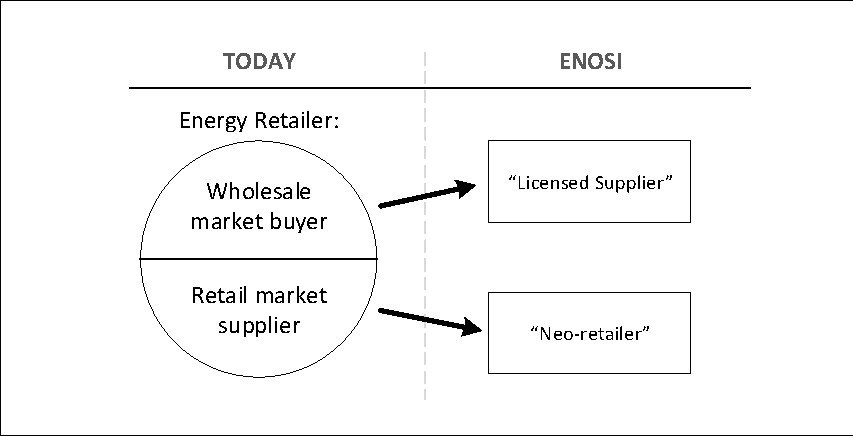
\includegraphics[width=250pt]{enosi-retailer-split}\\
\caption{Splitting of the traditional retail energy business.}\label{fig1}
\end{center}
\end{figure}

The Enosi platform, in essence, brings Licensed Retail Suppliers, Neo-Retailers, and consumers together to eliminate current structural inefficiencies and benefit all the parties. The platform consists of free software, but encapsulates its value with an associated Network-as-a-Token model. The initial funding of the Enosi platform build will be through an ICO of an ERC20 token, the \textit{Joul}, as a representation of the value of the Enosi network. The \textit{Joul} economically incentivises the network participants to inter-operate with each other to reinforce and grow the benefits that arise from the existence of the Enosi network. The Enosi software will be made open source and the \textit{Joul} is required to access individual energy networks in the Enosi platform. 
% * <matt.hale@block8.io> 2018-08-10T03:15:11.567Z:
% 
% > incentivises the network participants to inter-operate with each other to support the benefits that arise from the existence of the Enosi network
% I don't understand this sentence, do we mean to "reinforce the benefits" or "grow the benefits" perhaps?
% 
% 
% ^ <matt.hale@block8.io> 2018-08-17T05:02:30.707Z.


\newpage

\section{The Enosi Platform}
% * <matt.hale@block8.io> 2018-08-17T05:14:42.977Z:
% 
% > With the rise of distributed energy resources, including solar cells, batteries, and responsive demand devices, the opportunity has emerged to institute schemes that reduce inefficient grid capital investments. Placing generation resources closer to the demand reduces the need for long-haul transmission lines and electricity distribution infrastructure required to move power from large, centralised generation stations to the load.
% > % * <matt.hale@block8.io> 2018-08-10T05:03:29.632Z:
% > % 
% > % > from centralised generation stations to the load.
% > % "from large, centralised generators to the load."
% > % 
% > % ^ <matt.hale@block8.io> 2018-08-17T05:08:27.108Z.
% > % * <matt.hale@block8.io> 2018-08-10T05:02:45.489Z:
% > % 
% > % > closer to the source of power demand
% > % closer to the demand
% > % 
% > % ^ <matt.hale@block8.io> 2018-08-17T05:08:40.353Z.
% > % * <matt.hale@block8.io> 2018-08-10T05:02:13.486Z:
% > % 
% > % > Putting
% > % Placing
% > % 
% > % ^ <matt.hale@block8.io> 2018-08-17T05:09:02.068Z.
% > % * <matt.hale@block8.io> 2018-08-10T03:18:14.259Z:
% > % 
% > % > the opportunity has emerged to institute schemes that has a potential to reduce inefficient grid capital investments
% > % We need to rework this sentence, it doesn't flow well
% > % 
% > % 
% > % ^ <matt.hale@block8.io> 2018-08-17T05:10:41.572Z.
% > % * <matt.hale@block8.io> 2018-08-10T03:17:36.769Z:
% > % 
% > % > rise
% > % proliferation?
% > % 
% > % ^ <matt.hale@block8.io> 2018-08-17T05:10:50.884Z.
% > Enosi's model provides financial and community-based value incentives for such decentralisation of energy resources.
% 
% I do not understand why this content has been placed here. It was originally intended to provide context around the nature of Gird2.0, it seems very out of place here. I would include it in the introduction, or remove it. So much context has been lost because of this restructuring
% 
% ^ <matt.hale@block8.io> 2018-08-17T05:17:08.038Z.
With the rise of distributed energy resources, including solar cells, batteries, and responsive demand devices, the opportunity has emerged to institute schemes that reduce inefficient grid capital investments. Placing generation resources closer to the demand reduces the need for long-haul transmission lines and electricity distribution infrastructure required to move power from large, centralised generation stations to the load.
Enosi's model provides financial and community-based value incentives for such decentralisation of energy resources.

Enosi puts the end customers' needs and satisfaction at the forefront of its platform design by implementing structural efficiency to the benefit of all system actors. On occasion, however, grid owners will make much fanfare about deploying a trial of the latest engineering innovation that may indeed have potential to reduce their capital expenditure. Examples include smart metering, demand management systems and other `smart grid' technologies. Regulators and consumers alike should be frustrated by the fact that such trials so often remain just that - a trial, and an excuse to delay meaningful change on the grounds of prudence. Today, some twenty years after the successful deployment of two-way smart metering systems, utilities are still proposing pilots to trial technologies proven decades ago. This decentralised change has been described as the shift towards ``Grid 2.0" and attempts to sell innovative platforms that are intended to enable capital reductions in power grids are likely to be met with opposition (or worse, false enthusiasm) by the incumbents. Instead, Enosi's main goal is to eliminate the current structural inefficiencies through an automated network to empower consumers and communities.

The key to unlocking value in traditional energy markets is to reconfigure them with a different set of actors who can interact in a fundamentally more efficient way. We propose decomposing the traditional energy retailer into two distinct parts: a wholesale market facing Licensed Retail Supplier and a customer facing Neo-Retailer.

\noindent \textbf{\textit{Licensed Retail Supplier}} is a company or not-for-profit entity who buys electricity from the wholesale market and sells it into the retail market, typically via a Neo-Retailer. They are required to abide by existing prudential regulations, including holding capital to protect creditors (electricity generation businesses) against a failure of their credit risk operations.

\noindent \textbf{\textit{Neo-Retailer}} is a company or not-for-profit entity who specialises in providing customer-facing services, including customer acquisition, metering, billing, and ancillary services such as peer-to-peer energy functions. Neo-Retailers do not require an electricity market license and may be operated by anyone, including not-for profit community groups or tangentially related business (such as electric vehicle manufacturers) who can market more specific value propositions to their customers.

Such a decomposition of traditional energy retailers in the novel automated energy market ecosystem offers various benefits to both Licensed Retail Suppliers and Neo-Retailers, and ultimately to end customers. The Enosi platform will: 
\vspace{-1em}
\begin{itemize}
\item{create a single marketplace for Licensed Retail Suppliers to acquire customers and for Neo-Retailers in turn to publicly advertise and on-sell their unique, aggregated customer load profile to Licensed Retail Suppliers;}
\item{reduce the cost of customer management by supporting not-for-profit entities to act as Neo-Retailers since such entities will be structurally more competitive than traditional for-profit service companies, resulting in cheaper electricity prices for end-customers;}
\item{create a more diverse set of Neo-Retailers satisfying the specific needs of customer subgroups;}
\item{accelerate the use of smart metering as Neo-Retailers can form around this technology to offer even cheaper and more efficient retailing services by removing the need for manual meter-reading;}
\item{accelerate the use of distributed generation (e.g. rooftop solar) as it becomes easier for actors to enter the market and offer peer-to-peer services.}
\end{itemize} 


% * <matt.hale@block8.io> 2018-08-17T05:22:48.874Z:
% 
% >  On occasion, however, grid owners will make much fanfare about deploying a trial of the latest engineering innovation that may indeed have potential to reduce their capital expenditure. Examples include smart metering, demand management systems and other `smart grid' technologies. Regulators and consumers alike should be frustrated by the fact that such trials so often remain just that - a trial, and an excuse to delay meaningful change on the grounds of prudence. Today, some twenty years after the successful deployment of two-way smart metering systems, utilities are still proposing pilots to trial technologies proven decades ago. This decentralised change has been described as the shift towards ``Grid 2.0" and attempts to sell innovative platforms that are intended to enable capital reductions in power grids are likely to be met with opposition (or worse, false enthusiasm) by the incumbents. Instead, Enosi's main goal is to eliminate the current structural inefficiencies through an automated network to empower consumers and communities.
% 
% This might serve us better being further up in the section, say after the first paragraph. 
% 
% ^ <matt.hale@block8.io> 2018-08-21T00:48:56.937Z.
% * <matt.hale@block8.io> 2018-08-10T05:22:01.726Z:
% 
% > and other `smart grid' automation
% There's a word or two missing here at the end, not sure what though...
% 
% ^ <matt.hale@block8.io> 2018-08-17T05:20:13.262Z.
% * <matt.hale@block8.io> 2018-08-10T05:20:56.582Z:
% 
% > by aiming to benefit all the system actors through structural efficiency.
% "by implementing structural efficiency to the benefit of all system actors"
% 
% ^ <matt.hale@block8.io> 2018-08-17T05:23:42.757Z.

\enlargethispage{-1\baselineskip}
%This enables Licensed Suppliers to compliment their sell profile in order to optimise their buying profile, and in turn offer more competitive pricing to the Neo-retailer.
% * <matt.hale@block8.io> 2018-08-10T05:26:46.410Z:
% 
% > This enables Licensed Suppliers to compliment their sell profile in order to optimise their buying profile, and in turn offer more competitive pricing to the Neo-retailer.
% Why have we removed this? It seems pretty important
% 
% ^ <matt.hale@block8.io> 2018-08-21T00:47:02.703Z.

Creating such a network is made possible by using distributed ledger technology to efficiently share metering and customer data by also adhering to a common standard for the energy retailing stack. Having all market actors running a common software to standardise energy data (e.g., metering) and logic (e.g., billing) means that inter-operation between market players becomes possible. It would be impractical to integrate every disparate system that currently exists together, or create a separate for-profit company dedicated to interfacing between them all. It is only via the creation of a not-for-profit \textemdash\, Enosi \textemdash\, foundation, run by individuals who are incentivised to improve the value of the network, enables such a singular network to become possible. 
% * <matt.hale@block8.io> 2018-08-20T05:29:11.458Z:
% 
% > \textemdash\, Enosi \textemdash\
% I personally don't like this formatting, was it put here for a specific reason?
% 
% ^.
% * <matt.hale@block8.io> 2018-08-10T05:25:52.276Z:
% 
% > Creating such a network is achievable by using distributed ledger technology
% "Its possible to create such a network by using distributed ledger technology...."
% 
% ^ <matt.hale@block8.io> 2018-08-17T05:24:28.257Z.

Enosi is therefore tasked with building the software that enables the interactions of participants. Figure \ref{fig2} illustrates the separation of Licensed Retail Suppliers and Neo-Retailers in the energy stack. The separation simultaneously allows Neo-Retailers to offer energy services at reduced cost and enables Licensed Retail Suppliers to more effectively hedge their wholesale risk by accessing the aggregated load profiles of consumers. In the Enosi system, generators continue to their current roles, whereas the continuous cooperation between Licensed Retail Suppliers and Neo-Retailers, and the competition between Neo-Retailers enables the system to add value for consumers and communities. 
% * <matt.hale@block8.io> 2018-08-10T06:20:34.656Z:
% 
% > The separation simultaneously allows the Neo-Retailers reduce the cost stack 
% Not sure what is being said here, reducing the Neo's cost stack?
% 
% ^ <matt.hale@block8.io> 2018-08-17T05:27:15.264Z:
% 
% It doesn't follow that because we separate the actors that the Neo's cost stack is reduced... They didn't exist before. 
%
% ^ <matt.hale@block8.io> 2018-08-17T05:27:17.022Z.

\begin{figure}[h!]
% * <matt.hale@block8.io> 2018-08-20T05:30:30.673Z:
% 
% > \begin{figure}[h!]
% > \begin{center}
% > 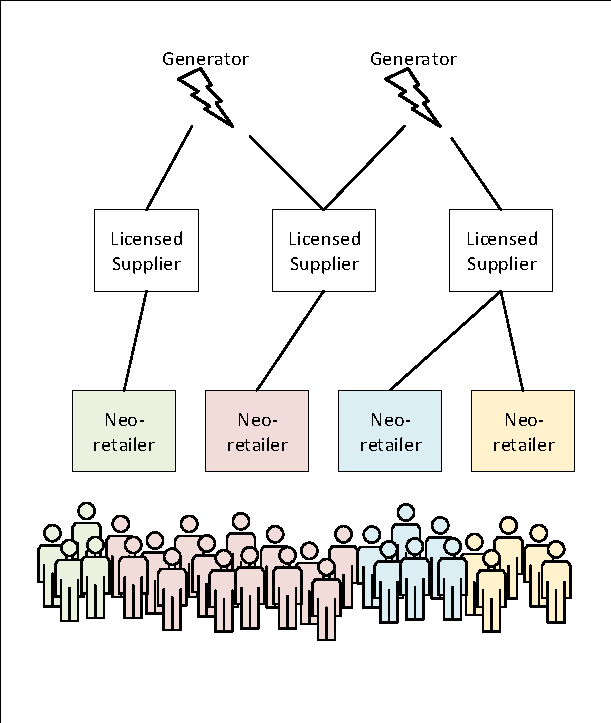
\includegraphics[width=250pt]{enosi-stack}
% > \caption{Separation of licensed and retail entities in the energy stack.}\label{fig2}
% > \end{center}
% > \end{figure}
% We should really use a better diagram from the whitepaper, not sure how to add one here myself
% 
% 
% ^.
\begin{center}
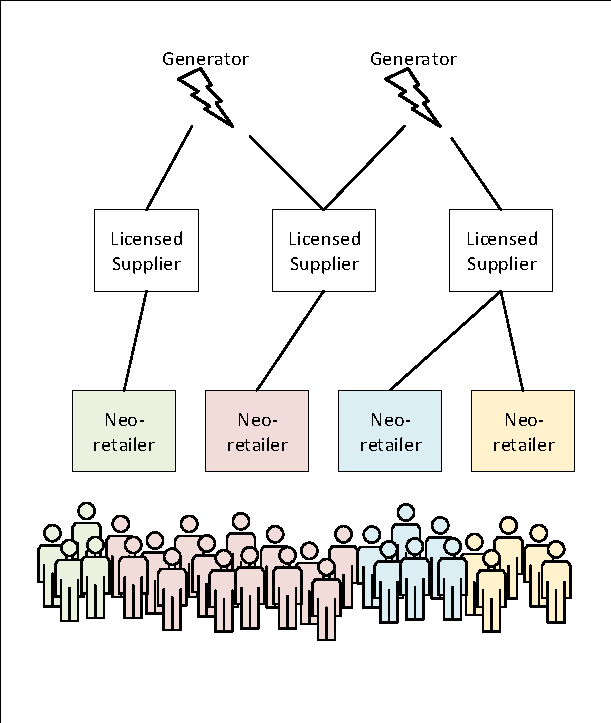
\includegraphics[width=250pt]{enosi-stack}
\caption{Separation of licensed and retail entities in the energy stack.}\label{fig2}
\end{center}
\end{figure}

As the network grows and matures over time, it is expected to create second-order incentives for Licensed Retail Suppliers to cooperate (and ultimately aggregate into super-operators) in order to continue to take advantage of sell-side aggregation of load profiles. Figure \ref{fig3} illustrates the fact that this network will naturally dissolve to a fragmented market through an increasing number of cooperative agreements. Because Neo-Retailers are in custody of their own data and logic (including a customer identity) and should be able to easily switch between their electricity supplier, the Enosi configuration is ideal for fostering the competition through cooperation with the system participants. 
% * <matt.hale@block8.io> 2018-08-10T06:23:33.103Z:
% 
% > and able to easily switch between their electricity supplier
% We need to checksum this, I don't think it will be quick to switch customers over to new LRS, it's a regulatory problem
% 
% Perhaps "should be able to switch..." would be better?
% 
% ^ <matt.hale@block8.io> 2018-08-21T00:49:25.546Z.
% * <matt.hale@block8.io> 2018-08-10T06:22:03.864Z:
% 
% > As the network grows and matures over time, it is expected to create second-order incentives for Licensed Retail Suppliers to cooperate (and ultimately aggregate into super-operators) in order to continue to take advantage of sell-side aggregation of load profiles. Figure \ref{fig3} illustrates the fact that this network will naturally dissolve to a fragmented market through an increasing number of cooperative agreements. 
% I am confused. In the first sentence we say large amounts of aggregation will take place and in the very next sentence we say that the network will dissolve into a fragmented market  - are these two not inherently contradictory? Or am I missing something?
% 
% ^.


\begin{figure}
\begin{center}
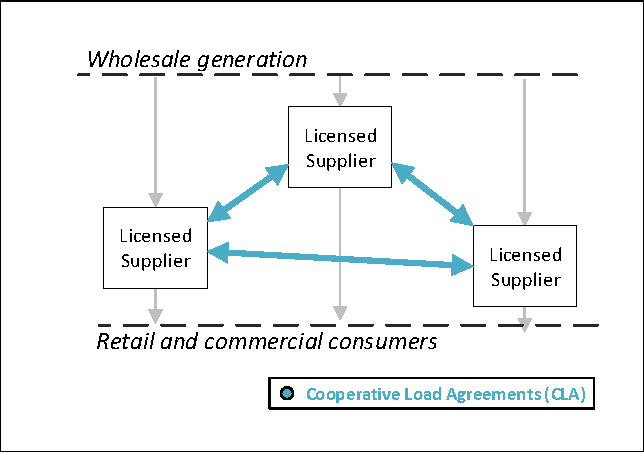
\includegraphics[width=250pt]{enosi-cla}
\caption{Financial agreements between wholesale energy traders.}\label{fig3}
\end{center}
\end{figure}

The ultimate arrangement of the Enosi network within a given market is the maximal connectivity between Licensed Retail Suppliers and Neo-Retailers who follow their economic incentives. Once this process reaches its equilibrium, the end-state of the network will effectively become a Distributed Autonomous Organisation (DAO) functioning as a wholesale market player that is owned and governed by community members and Neo-Retailers. In this end state, the regulatory environment will be ready to be reformed to bring wholesale buying into the ecosystem as well. In this scenario, the various aggregated wholesale buying entities will be replaced by a single DAO, per wholesale jurisdiction, that would handle all the wholesale market interactions on behalf of the Neo-Retailers. At this point in time, the way energy is procured and distributed to Neo-Retailers and eventually to end-consumers is run entirely for the community via market Enosi DAOs (EDAO). The Enosi project is breaking apart the existing inefficient model and rebuilding it with the community at the centre. The cryptoeconomic incentive scheme supporting this network, including the use of the \textit{Joul} to represent network's value is described in the next section. We conclude this section by summarising the Enosi actors, their roles, and the trust structure among them. 
% * <matt.hale@block8.io> 2018-08-10T06:25:44.538Z:
% 
% > Enosi DAOs (EDAO)
% Does it matter here that we are conflating the idea of having a Retailing entity run as a DAO (EDAO) with the idea that one day you could have a wholesale market entity which is a DAO?
% 
% ^ <matt.hale@block8.io> 2018-08-20T05:35:23.029Z:
% 
% We talk of a singular wholsale DAO here but in the table below talk of EDAOs as Neo-Retailers without central governance
%
% ^.
% * <matt.hale@block8.io> 2018-08-10T06:24:51.954Z:
% 
% > by community members
% and possibly Neo Retailers too
% 
% ^ <matt.hale@block8.io> 2018-08-20T05:35:46.316Z.

\subsection*{Enosi actors} A summary of the various Enosi actors, their roles and motivations in the Enosi ecosystem are tabulated below in Table \ref{tab}. The actors' roles and motivations in the system are important to understand the trust structure among them, and ultimately design economic incentive mechanisms to achieve the objectives of the Enosi platform. 


\newpage


\begin{landscape}
\begin{center}
\begin{tabular}{|l|l|l|}
 \hline 	
\textbf{Enosi Actor} & \textbf{Motivations and use of Joul}\\
 \hline 
 \hline
 \textbf{Enosi Foundation} - Facilitator of Enosi ecosystem. Manages the 	 	& Wants to build and maintain the infrastructure required to support the Enosi network.			\\
 staking function for the network.	 	&  Recieves a small fee in Jouls each time they are traded in the ecosystem. 		\\
 \hline 
  \textbf{Licenced Supplier} - Financially responsible market participant 		& Wants to access additional customers to obtain a better risk position on the wholesale		\\
   (FRMP), interacting with the wholesale energy market and supplier  	& 	 market. Stakes Jouls in order to access the Enosi network.		\\
	to the retail market.		& 		\\
 \hline 
  \textbf{Neo-retailer} - Entity providing a consumer interface to the wholesale	& Wants to facilitate Grid 2.0 energy services to customers with their unique value  	\\
  market, including billing and exception management functions. 		&   proposition. Stakes Jouls in order to access the Enosi network.			\\
 \hline 
 \textbf{Application Provider} - Third party offering services to actors in	the & Wants to provide goods and services to  actors in the Enosi network. Currently, no  		\\
   Enosi  network, such as a metering data provider.				& need to acquire Jouls to pariticpate. \\
 \hline
 \textbf{EDAO} - Enosi Decentralised Autonomous Organisation. Functions			& Acts only as programmed. Jouls sourced by	members are used to stake for the	\\
like a neo-retailer	without central governance. 	&  continued participation in the network.	\\
 \hline
\textbf{Consumer} - Consumer/prosumer of  energy who is a member of a 	 		& Wants cheaper electricity and the ability to trade directly with peers. Procures Jouls 	\\
neo-retailer or EDAO.		& to directly participate in the network within a DAO, or joins as a member of a 	\\
  								&  neo-retailer who procures Joul on their behalf. 		\\
 \hline
\end{tabular}
\end{center}
\vspace{+1em}
\captionof{table}{A summary of the Enosi actors, their roles and motivations.}\label{tab}
\end{landscape}


\subsection*{Trust structure}

To develop smart contracts between the defined actors, we must understand which of those actors are in a natural financial contention. That is, for which actor pairs do we need to write trust management programs into the Enosi permissioned distributed ledger system? We therefore contrast the current trust relationships in the energy markets and Enosi's automated trust structure in terms of four important characteristics of the system. 

\vspace{+1.5em}

\begin{mdframed}
\centering
\textbf{1. Accuracy and fairness of billing}
\end{mdframed}

\begin{mdframed}

\noindent \textbf{Current}: Customers trust that billing is accurate and fair between them and their licensed retailer. 

\noindent \textbf{Enosi}: A permissioned distributed ledger is used to prove the calculation of the customer’s electricity bill.

\end{mdframed}
\vspace{+1.5em}

\begin{mdframed}
\centering
\textbf{2. Reliability of energy supply}
\end{mdframed}
\begin{mdframed}

\noindent \textbf{Current}: Customers trust that their licensed supplier will reliably supply them with energy from the wholesale market. Generators trust that retail license holders will accurately and effectively settle the `overs and unders' between the wholesale market and the downstream markets.

\noindent \textbf{Enosi}: Customers and neos trust that their licensed retailer will reliably supply them with energy from the wholesale market. Neos will accurately and effectively settle the demand of the downstream markets.

\end{mdframed}
\vspace{+1.5em}

\begin{mdframed}
\centering
\textbf{3. Security and veracity of data}
\end{mdframed}
\begin{mdframed}

\noindent \textbf{Current}: Customers trust that their data is kept secure and is accurately maintained. 

\noindent \textbf{Enosi}: All Enosi participants can verify the veracity of data. Customers have control over the accuracy and permission of their data. Data resides encrypted on a permissioned distributed ledger and customers provide permission for the storage of their data.

\end{mdframed}
\vspace{+1.5em}

\begin{mdframed}
\centering
\textbf{4. Trust on metering information}
\end{mdframed}

\begin{mdframed}

\noindent \textbf{Current}: All participants trust smart meters and meter data providers (MDPs) for metering information. 

\noindent \textbf{Enosi}: No change to the current market, however neo-retailers providing services to customers only with smart meters should result in cheaper pricing.

\end{mdframed}




\newpage

Hence, we can define the following transactional relationships more formally from the base actor types: licensed supplier, neo-retailer, and consumer.

\begin{itemize}

\item{ \textbf{Licensed Supplier - Licensed Supplier}:
In commercial competition. They do not wish to share any data, including metering data. However, smaller licensed suppliers may benefit from sharing anonymised metering data and jointly buying wholesale hedges to match the aggregated demand profile.}

\item{ \textbf{Licensed Supplier - Neo-retailer}:
Neo-retailer acts as a sales channel for a licensed supplier. Neo-retailer only provides minimum required information to the licensed supplier. Neo-retailer only links in with the licensed supplier to gain pseudo-access to a retail energy licence. Licensed supplier wishes to acquire customers through neo-retailers and may incentivise them to access to their retail energy licence via a marketplace on the Enosi platform.}

\item{ \textbf{Licensed Supplier - Consumer}:
Consumer wishes to reduce their costs, while the licensed supplier wishes to maximise profits. Consumer needs the licensed supplier to take away the wholesale risk.}

\item{ \textbf{Neo-retailer - Neo-retailer}:
May or may not be in commercial competition. Larger and more `commercial' neo-retailers may be in commercial competition in a similar fashion as two licensed suppliers.}

\item{ \textbf{Neo-retailer - Consumer}:
In some scenarios, a consumer may wish to reduce their costs, while a neo-retailer may wish to maximise profit. In others, a consumer may wish to contribute to the community, while a neo-retailer may wish to facilitate consumer contributions to the community.}

\item{ \textbf{Consumer - Consumer}:
There may be concerns that other consumers are bad actors wanting to exploit their data if shared with others. However, some communities might have a higher level of inherent trust than others and will share data with permissions.}

\end{itemize}


Other key elements to the inter-operation of these actors include \textit{identity standards for all standard actor types} (e.g., a fully-featured consumer identity that satisfies the requirements of licensed suppliers, neo-retailers, and other consumers), \textit{interfaces for external actors} (e.g., regulators to interact with the system), \textit{standarised software for basic operational tasks} (e.g., an interface to the load profile market, customer onboarding, billing and settlement functions). 




\newpage
\enlargethispage{-1\baselineskip}

\section{Network-as-a-Token: Joul}
In this section, we discuss the value of the Enosi network for different network participants, how the \textit{Joul} represents the network's value, and the economic incentives of the network participants to inter-operate. 

\subsection*{Value of the Enosi network} Blockchains are good at representing value as they resolve the double-spend problem for both digital assets and digital representations of real-world assets. All value in any asset is fundamentally derived from a network of participants with mutual beliefs. While ``real-world assets" derive their value from existing markets and agreed utility established over time, ``crypto-assets" do not benefit from the tenure of well-known markets established over time. They, however, derive value from a network of participants who collectively agree on the value that the token represents. For Enosi, we define the value of the Enosi platform for different actors to be the following.
\vspace{+1em}

\noindent For Licensed Retail Suppliers;
\begin{itemize}
\item{A means to access benefits of scale, including minimising wholesale buying risk.}
\item{A means to access a pool of new energy customers.\\}
\end{itemize}
\vspace{-1.5em}

\noindent For Neo-Retailers;
\begin{itemize}
\item{The ability to provide specialised retail services without a retail energy licence.}
\item{A means to access a marketplace of energy retailers and energy consumers.
The ability to access energy retail business software, including billing and metering processes.\\}
\end{itemize}
\vspace{-1.5em}

\noindent For consumers and prosumers;
\begin{itemize}
\item{Minimised electricity prices due to cooperative load agreements.}
\item{The means to undertake peer-to-peer energy trading.}
\item{The ability to be in better control on where you buy your power from.}
\item{The ability to have control your metering data and visibility of your billing logic.}
\item{The ability to act as your own energy retailer, ("Neo-retailer"), and cooperate with others to form a decentralised autonomous organisation (EDAO).}
\item{The ability to efficiently change electricity retailers.\\}
\end{itemize}

\noindent For all Enosi actors;
\begin{itemize}
\item{Aggregated data useful for third party analytics.}
\item{Brand awareness of this particular platform.}
\item{An operating foundation supporting the development of this particular ecosystem.}
\item{A means to influence a greener and more decentralised energy future by incentivising the use of smart meters and distributed generation.}
\end{itemize}

Currently, community-based organisations cannot become energy retailers without first obtaining an energy retail license. Today, this is a prohibitively costly and cumbersome process. The Enosi ecosystem facilitates new and innovative models of community-oriented energy supply and management by providing the means to share energy-related data and logic. This also democratises access to energy retail licensing by enabling businesses specialising in wholesale risk management without the need to manage consumers. With the successful implementation of the Enosi ecosystem and the market efficiencies that are unlocked, the idea of a truly community-based energy retailer becomes possible.

\subsection{Representation of Enosi's value: Joul}
Now that we have defined the value of the Enosi network, we define a fungible cryptographically-secure token, the \textit{Joul}, which represents this value. We recognise the difficulty in representing all forms of value in tokenised form, including data and open source software. The main difficulty in tokenising Enosi data and software is that it can be freely copied and simply cannot have its value captured in the same way that a software licence can capture value. Therefore, in our value definition, we have not defined the software itself as part of the value represented by the token. For the Enosi network to operate, we have designed the \textit{Joul} to be an access token.\footnote{ There are a number of alternative token utility models that we considered to represent Enosi's value. First, \textit{tokenised electricity} is a poor candidate since electricity is not usually stored or owed. It is always bought/sold and then settlement occurs at a later time. Thus, there is rarely the situation where electricity can be held for value appreciation. In addition, the asset is ephemeral (it is typically only generated once and consumed once) and  difficult to transfer to a market outside the one in which it is geographically located. Second, \textit{settlement tokens} are also questionable to represent Enosi's value since they can cycle through the system very quickly. A high token velocity is problematic because there is no incentive to hold the token and incur price risk relative to other currencies (fiat or crypto). This is because in order to settle, one simply needs to buy the required quantity of tokens at settlement, thereby increasing sell pressure at all other times. Fundamentally, if there is no need for regular users to hold on to the token then the token’s price is only linked to speculation. Contrastingly, if everyone holds the tokens and no one is using them within the ecosystem or trading them outside of it, transactional volume collapses as does the price of the token because there is no demand.} 
\textit{Joul} is required to access the permissioned Enosi network and allow inter-operation with other network participants. 
Such a recursive scheme is a neat way of supporting the value of the Enosi network since its value is directly measurable in the open market. Enosi enforces network permissioning through the ‘staking’ of \textit{Jouls} within a smart contract on a public blockchain, such as Ethereum. Once the staking requirements of the smart contract have been satisfied, permission is provided for the owner of that stake to join the Enosi network. Permissioning is managed by the network consensus (initially, this will be managed by Enosi centrally).

\vspace{-0.3em}

\subsection*{Mechanics of the Joul}
The objective of the programming of the \textit{Joul} is to encourage the network cohesion. That is, the objective is to incentivise the defined market actors to continue to inter-operate with each other to support the benefits that arise from the existence of the network. The base mechanic of the \textit{Joul} to achieve Enosi's objective is a \textit{staking function}. Enosi requires both Licensed Suppliers and Neo-Retailers to stake \textit{Jouls} to participate in the network, depending on their measured ``size". A stake is not initially required for a startup or very small platform actors to join the Enosi network, but the required stake grows as a function of the number of customers connected to that particular actor. The staking function is based on the incremental cost per customer. More precisely, it is zero for a startup actor with zero connections and near-zero for a very small player, but eventually becomes more for larger actors to onboard new customers. This design effectively incentivises smaller participants to initiate their energy market endeavours on the Enosi platform and encourages a decentralised retailing model.

Formally, let $i\in\{f, l, n, a, d, c\}$ denote the participants within the Enosi ecosystem, where $f$ stands for the foundation, $l$ for Licensed  Retail Suppliers, $n$ for neo-retailers, $a$ for application providers, $d$ for DAOs, and $c$ for consumers. We define a staking function $S(C_i, T_i)$ for the actor $i$, where $C_i$ is the number of customers connected to the actor $i$ and $T_i$ is the tuning parameter for the Enosi foundation. The staking function calculates the required number of Jouls, $J$, to stake for access to the Enosi network per actor type. There are a number of desired properties for the staking function to satisfy for the efficient operation of the Enosi system. First, for the Enosi network to grow, the consumers ($c$) should not stake $J$ to participate in the Enosi platform. We therefore set $S(C_c, T_c) = 0$. Second, DAOs ($d$) are not a distinct actor type (it assumes another actor type) and the Enosi foundation ($f$) maintains the efficient operation of the Enosi platform. We therefore do not define a staking function for these actors and relegate the need to stake Jouls to other actors. Third, initially, the functions provided by application providers ($a$) will be provided by either the Licenced Retail Suppliers or Neo-Retailers. Thus, we focus our attention on the Licensed Retail Suppliers ($l$) and Neo-Retailers ($n$). 

For the efficient operation of the Enosi ecosystem, we aim for the network cohesion among the Licensed Suppliers ($l$) and Neo-Retailers ($n$). To achieve the ultimate network cohesion within the Enosi ecosystem, the staking function should satisfy two main properties. First, it should incentivise smaller market players to join the system and disincentivise larger market players to exit. That means the staking function should be zero for actors with zero customers (i.e., $S(0,T_i)=0$) and monotonically increasing in the number of customers $C_i$ connected to the actor $i$ (i.e., $\frac{\partial S(C_i,T_i)}{\partial C_i}>0$). Second, we want the incentive and disincentive mechanisms to be robust, so that the actors do not deviate from the main objective of Enosi. We therefore require the staking function to increase in the number of customers $C_i$ at an increasing rate (i.e., $\frac{\partial^2 S(C_i,T_i)}{\partial C_i^2}>0$). The second condition ensures that larger market players will refrain from sudden market disruptions, such as market exits. A simple exponential relationship, i.e.,
% * <matt.hale@block8.io> 2018-08-10T06:37:10.858Z:
% 
% > For the efficient operation of the Enosi ecosystem, we aim for the network cohesion among the Licensed Suppliers ($l$) and Neo-Retailers ($n$). To achieve the ultimate network cohesion within the Enosi ecosystem, the staking function should satisfy two main properties. First, it should incentivise smaller market players to join the system and disincentivise larger market players to exit. That means the staking function should be zero for actors with zero customers (i.e., $S(0,T_i)=0$) and monotonically increasing in the number of customers $C_i$ connected to the actor
% 
% There seems to be a 'double staking' requirement for each customer here. i.e. both the Neo and the LRS have to stake in order to service the same customer. 
% 
% We need to be a bit more specific about how the LRS staking condition differs from the Neo's staking condition -  some people are already asking us about this 'double staking' and how much it will cost each of these actors to access the network.
% 
% ^.
\begin{equation*}
S(C_i, T_i)=C_i^{(e\cdot T_i)}, 
\end{equation*}
satisfies both conditions when $T_i>\frac{1}{e}$. If a customer leaves the Licensed Retail Supplier or the Neo-Retailer, \textit{Jouls} escrowed within a stake are released. In practical terms, these actors will need to maintain a working balance as customers leave and join their organisations. Similarly, consumers who wish to participate in an EDAO are required to source \textit{Jouls} in order to pay for the EDAO stake to participate in the Enosi ecosystem.

The staking function, $S(C_i,T_i)$, in its current form determines the number of \textit{Jouls} to stake based on the number of customers, but can be further tuned for different customer types, including commercial customers, or total electricity consumption by the actor's connected customers. The staking rate for actors can be extended to more sophisticated incentive schemes to encourage network cohesion. For example, discounts on the required stake could be implemented for Licensed Retail Suppliers as a function of their purchased energy mix (i.e. how much sustainable power is being bought on the wholesale market) or Neo-Retailers as a function of how many smart meters are installed in their customer base. However, the staking function, $S(C_i,T_i)$, in its current form is simple enough to be understood by all the Enosi participants and adequate to capture the core incentive mechanism for the operations of Enosi.

Another important aspect of the mechanics of \textit{Joul} is the \textit{slashing condition} (i.e., the condition under which the actor loses the stake). Each participant on the Enosi platform has a value pool relative to their customer size in the network that remains at stake. The conditions under which an actor may have his stake slashed include 
\begin{itemize}
\item{connection to external networks,}
\item{data or privacy breach,}
\item{failure to provide customer data on request,}
\item{reasons as voted by network members.}
\end{itemize}
Slashed balances are either destroyed or appropriated by the Enosi Foundation to be spent on network-enhancing activities, such as smart meter subsidies within the same market.

Finally, for the Enosi model to be complete we provide the details of \textit{transaction fees} and \textit{rate adjustments}. 
To support the ongoing operational expenses for the Enosi foundation, \textit{a small fee} is to be levied on all \textit{Joul} transactions. Fees accumulated by the foundation are then sold back to Neo-Retailers, Licensed Retail Suppliers or other actors wishing to procure \textit{Jouls} on a decentralised exchange. In addition, \textit{fee and staking rates} are able to be adjusted by the Enosi Foundation. Such adjustments could be initiated for any reason in accordance with their mandate and include
\begin{itemize}
\item{a situation where market participation is becoming saturated using Enosi. In this scenario, a cap on the additional required stake might be included to prevent perverse punitive measures on larger organisations (e.g. avoiding situations where onboarding the last remaining customer requires an unnecessarily large stake).}
\item{a situation where the value of Joul becomes too great. This might create perverse incentives to de-leverage customers and release \textit{Jouls} for sale on the market. In this instance, the Foundation may elect to reduce the required stake to allow fees to be paid out of an actor’s stake if the value goes way above, but they would need to maintain a buffer on top of the minimum stake.}
\end{itemize}


\newpage

\section{Implementation}

In this section, we explore the implementation considerations for the Enosi ecosystem. We describe the possible approaches for implementing a distributed ledger technology, transaction limits of near-real-time smart meter oracles, initial settlement, and exception management.       

\subsection*{Distributed ledgers} There are three main candidate approaches for implementing a distributed ledger technology to achieve Enosi's goals; \textit{(i)} public gossip blockchain, \textit{(ii)} permissioned gossip blockchain, and \textit{(iii)} permissioned mesh distributed ledger.

\textit{(i) Public gossip blockchain} is implementation on an open, public blockchain infrastructure such as Ethereum or EOS. In this scenario, all Enosi transactions would be public, including sensitive transactions relating to customer energy usage or customer bill payments.\footnote{ There are privacy technologies such as private transactions using encrypted smart contract state that may be available in the future. However, these are beyond the immediate implementation timeline.} Public gossip blockchain is also associated with significant scalability challenges which make it undesirable for Enosi. \textit{(ii) Permissioned gossip blockchain} is implementation of a gossip-style blockchain, but with higher transaction throughput and a permissioned validator set. A permissioned chain sacrifices some security in return for performance. Such an implementation is able to access much higher transaction throughput than a public gossip blockchain and incurs a performance overhead from incorporating private transactions. Although the criticality of the information being protected is only moderate, and goes stale over some time period, the privacy leakage combined with the performance impacts also renders a permissioned gossip blockchain a less-than-ideal option.

\textit{(iii) Permissioned mesh distributed ledger} is a distributed ledger network where individual actors connect using a standard set of smart contracts. This scenario has the highest data privacy model as no private data is shared beyond the required participants, even in encrypted form. Transaction throughput is also high relative to the two aforementioned options as there is far less transaction overhead with a configurable connection mesh (nodes only connect to those nodes they are doing business with). Types of technologies with these properties include IBM's Hyperledger and R3's Corda. Due to the private nature of customer energy data, scalability constraints of current public blockchains, and the natural topology of the energy market (acyclic graph), a permissioned mesh network is the most appropriate architecture for Enosi. Hence, to maximally preserve data privacy, the state of various actors is isolated from other actors when they do not explicitly share a smart contract. For example, the isolation may occur between two customers or between a customer and a foreign licensed supplier. Note, however, that this requires a separate service to validate the uniqueness of unspent transaction outputs, such as the \textit{Notary function} in Corda.

\enlargethispage{-0.5\baselineskip}

\subsection*{Transaction volume}
We now consider the transaction throughput of several neo-retailers connected to different magnitudes of end-consumers and neo-retailers operated as DAOs to highlight the transactional limits of near-real-time smart meter oracles. The analysis provides an indication of the required transactions per second (i.e., $t/s$) for a given number of concurrent customers and a given smart meter data latency. Smart meter oracle injecting information into shared state is assumed to be a low-impact transaction with high-frequency.\footnote{ To make the analysis clear, we ignore low-frequency, high-impact transactions such as billing operations and other customer operations as well as compounding factors such as peer-to-peer energy trades, in which complex trades can generate multiple transactions per time interval.} 

For a \textit{centralised neo-retailer} connected to numerous customers (star graph topology), certain configurations of data latency and concurrent customers reach extremely high transaction throughput. Given Corda's recent scalability figures, Table \ref{tab2} shows that a neo-retailer with 200,000 customers can expect a smart meter data latency of no better than 1 minute, while a neo-retailer with 5,000,000 customers can expect no better than 30 minutes.\footnote{ See, for example, \textcolor{blue}{\href{https://medium.com/corda/transactions-per-second-tps-de3fb55d60e3}{https://medium.com/corda/transactions-per-second-tps-de3fb55d60e3}}.}
\vspace{+1em}
\begin{center}
\begin{tabular}{|l|l|l|l|l|}
 \hline 	
 \textbf{Interval} 		& \textbf{1s} & \textbf{1min} & \textbf{5min} & \textbf{30min}\\
 \hline 
 \hline
 1,000 customers:		& 1k $t/s$	& 17 $t/s$	& 3 $t/s$		& 1 $t/s$ \\
 200,000 customers:		& 200k $t/s$	& \textbf{3.3k} $t/s$	& 667 $t/s$	& 111 $t/s$ \\
 5,000,000 customers:	& 5M $t/s$	& 83k $t/s$	& 17k $t/s$	& \textbf{2.8k} $t/s$ \\
 \hline
\end{tabular}
\vspace{+1em}

\captionof{table}{Transaction throughput of a centralised neo-retailer.}\label{tab2}
\end{center}

For a \textit{decentralised neo-retailer} \textemdash \, DAO operating as a neo-retailer \textemdash \, (fully connected graph topology), we quickly run into transactional limits as illustrated in Table \ref{tab3}. Assuming quadratic transaction scaling, we run into transactional limits with fully connected DAOs with an upper-limit of around 1,000 actors and a 5 minute data latency. While transaction frequency will become very high for customers seeking near-real-time performance, a typical customer should only need at most around 50MB of metering data per year.

\vspace{+1em}

\begin{center}
\begin{tabular}{|l|l|l|l|l|}
\hline 	
 \textbf{Interval} 		& \textbf{1s} & \textbf{1min} & \textbf{5min} & \textbf{30min}\\
 \hline 
 \hline
 
 10 actors:		& 100 $t/s$	& 1.6 $t/s$	& 0.3 $t/s$	& 0.06 $t/s$ \\
 100 actors:	& 10k $t/s$	& 166 $t/s$	& 33 $t/s$	& 5.5 $t/s$ \\
 1,000 actors:	& 1M $t/s$	& 16k $t/s$	& \textbf{3.3k} $t/s$	& 555 $t/s$ \\
 10,000 actors:	& 100M $t/s$	& 1.6M $t/s$	& 333k $t/s$	& 55k $t/s$ \\
 \hline
 
\end{tabular}
\vspace{+1em}

\captionof{table}{Transaction throughput of a decentralised neo-retailer.}\label{tab3}
\end{center}

\subsection*{Settlement}
We initially plan to use regular banking rails until the widespread adoption of \textit{Joul} and the resolution of the problems associated with user onboarding and private key management are solved. This means that Neo-Retailers will hold credit risk in relation to their customers not paying for the electricity they use and a separate billing function administered on traditional payment rails. Alternatives to this include Neo-Retailers offering discounts for customers who pre-pay or modeling fiat currency on-ledger as a claim to cash held in a bank account. Ultimately, the Enosi ecosystem may interface with cryptocurrency payment rails or integrate into national fast payments networks. We may also see the implementation of national cryptocurrencies or similar programmable money as an alternative that can be used for ``on-chain" real-time settlement and thus reduce the price of power even further for end-consumers.

\subsection*{Exception management}

Customer exception management is the processing of customers who encounter an issue that is outside of the normal business processes such as sign-up and monthly billing. The number of exceptions dealt with by a Neo-Retailer limits the maximum size to which they can feasibly grow. 
It becomes increasingly difficult and expensive to deal with the exceptions. Hence, we foresee that these exceptions will be sufficiently distributed across all Neo-Retailers. Therefore, we are able to gain the benefits of larger players whilst retaining the agility and lightness of Neo-Retailers. If a Neo-Retailer grows to a more significant customer base, this will necessitate a greater investment into the exception process. While this will become easier with maturing technology over time, it is beyond the scope of the business process primitives that Enosi will be providing.

%\subsection{Example implementations}

%\textbf{ACME Electric Cars}\\

%\noindent Bought a new electric car? Access the network for free and gain full transparency over how your vehicle is charged, or have ACME pay your electricity for the life of the vehicle.\\

%\noindent \textbf{Bondi Locals Community}\\

%\noindent Dave, a Bondi local, retired electrical engineer and surfer, cares about the environment and his two grandchildren who attend the local public school. He starts a community group through the school to setup a local energy retailer. 

% \pagebreak
% \subsection{Roadmap}

% Description of key ecosystem functions changing over time:

% Function
% Now
% Day 1 
% Grid 2.0
% Settlement
% Quarterly billing from meter data in fiat by Retailer.
% Quarterly billing from meter data in fiat by Neo Retailer.
% Real time settlement of trades in a stable coin via the blockchain.
% Customer Onboarding and Management
% Managed entirely by Retailer.
% Managed by Neo Retailer.
% Managed by Neo Retailer.
% Accounts
% Managed entirely by the Retailer. Users can switch, but is difficult.
% Managed entirely by the Neo Retailer. Users can easily switch.
% Managed entirely by the user’s DApp, they have full autonomy.
% Customer ‘Control’
% Virtually none. No transparency.
% Increased choice about how your energy is sourced and sent. Increased transparency.
% Complete choice about how your energy is sourced and sent. Complete transparency.
% P2P Energy Trading
% Heavily involves centralised parties.
% Involves centralised parties in a greatly reduced capacity.
% P2P trading is completely decentralised.



\newpage


\section*{Work ahead}

We believe that \textit{sustainable, decentralised generation and consumption} is the future of electricity. This is where the retailers become the wholesalers; electricity that is generated from homes powers businesses during the day and distributed battery storage for the entire grid, where most of our energy needs can be met with renewables, distributed generation and storage. In such a distributed future, the most efficient transport of electricity is actually determined by physical location. As a node in the network attempts to satisfy a power deficit, it can immediately draw upon any local batteries that are currently advertising a surplus. In this model, power is actually purchased based on both location and price.

%Nodes will hold balances and be able to make purchase and sale decisions based on some predefined rules. The speed of such a system would need to be very fast, and communicate over very reliable networks, however should always default to a known value in case of communication failure.

Enosi's model is a step toward this future. In this model, the grid operators are encouraged to participate in local community markets which offer financial incentives to the owners of distributed resources to take actions aimed at optimising grid conditions and reducing overall costs for all. In the future, such a peer-to-peer trading system may benefit from the tokenisation of stored power. However, security challenges relating to how tokens are generated and decay (power generation and storage) lie ahead of us.

Another important area of future work is extending the current baseline mechanism design. Although, the current incentive scheme is simple and adequate to maintain efficient inter-operation of the Licensed Retail Suppliers and Neo-Retailers, we aim to extend the baseline design along two different dimensions. First, we aim to extend the current staking of Licensed Retail Suppliers and Neo-Retailers to take different customer types or total electricity consumption of connected customers into account. Second, and importantly, we aim to add other actors such as \textit{meter data providers}, \textit{exception processing providers}, and \textit{data merchants} who wish to purchase Neo-Retailer's aggregated data or underlying customer data into our baseline design to achieve Enosi's goals. %Any profits from this can flow down to the customer or be retained by the neo-retailer.




\end{document}

